\subsection{Linux kernel sources}

\begin{frame}
  \frametitle{Location of official kernel sources}
  \begin{itemize}
  \item The mainline versions of the Linux kernel, as released by Torvalds
    \begin{itemize}
    \item These versions follow the development model of the kernel
          (\code{master} branch)
    \item They may not contain the latest developments from a specific
      area yet
    \item A good pick for products development phase
    \item \url{https://git.kernel.org/pub/scm/linux/kernel/git/torvalds/linux.git}
    \end{itemize}
    \item The stable versions of the Linux kernel, as maintained by a
      maintainers group
    \begin{itemize}
    \item These versions do not bring new features compared to Linus'
      tree
    \item Only bug fixes and security fixes are pulled there
    \item Each version is stabilized during the development period of
      the next mainline kernel
    \item Certain versions can be maintained for much longer, 2$+$ years
    \item A good pick for products commercialization phase
    \item \url{https://git.kernel.org/pub/scm/linux/kernel/git/stable/linux.git}
    \end{itemize}
  \end{itemize}
\end{frame}

\begin{frame}
  \frametitle{Location of non-official kernel sources}
  \begin{itemize}
  \item Many chip vendors supply their own kernel sources
    \begin{itemize}
    \item Focusing on hardware support first
    \item Can have a very important delta with mainline Linux
    \item Sometimes they break support for other platforms/devices
      without caring
    \item Useful in early phases only when mainline hasn't caught up yet
      (many vendors invest in the mainline kernel at the same time)
    \item Suitable for PoC, not suitable for products on the long term
      as usually no updates are provided to these kernels
    \item Getting stuck with a deprecated system with broken software
      that cannot be updated has a real cost in the end
    \end{itemize}
  \item Many kernel sub-communities maintain their own kernel, with
    usually newer but fewer stable features, only for cutting-edge
    development
    \begin{itemize}
    \item Architecture communities (ARM, MIPS, PowerPC, etc)
    \item Device drivers communities (I2C, SPI, USB, PCI, network, etc)
    \item Other communities (real-time, etc)
    \item Not suitable to be used in products
    \end{itemize}
  \end{itemize}
\end{frame}

\begin{frame}
  \frametitle{Getting Linux sources}
  \begin{itemize}
  \item The kernel sources are available from
    \url{https://kernel.org/pub/linux/kernel} as {\bf full tarballs}
    (complete kernel sources) and {\bf patches} (differences between
    two kernel versions).
  \item But today the entire open source community has settled in favor
    of Git
    \begin{itemize}
    \item Fast, efficient with huge code bases, reliable, open source
    \item Incidentally written by Torvalds
    \end{itemize}
  \end{itemize}
\end{frame}

\begin{frame}
  \frametitle{Going through Linux sources}
  \begin{columns}
    \column[t]{0.4\textwidth}
    \begin{itemize}
    \item Development tools:
      \begin{itemize}
      \item Any text editor will work
      \item Vim and Emacs support ctags and cscope and therefore can help
        with symbol lookup and auto-completion.
      \item It's also possible to use more elaborate IDEs to develop
        kernel code, like Visual Studio Code.
      \end{itemize}
    \end{itemize}
    \column[t]{0.6\textwidth}
    \begin{itemize}
    \item Powerful web browsing: Elixir
      \begin{itemize}
      \item Generic source indexing tool and code browser for C and C++.
      \item Very easy to find symbols declaration/implementation/usage
      \item Try out \url{https://elixir.bootlin.com}!
      \end{itemize}
    \end{itemize}
    \begin{center}
      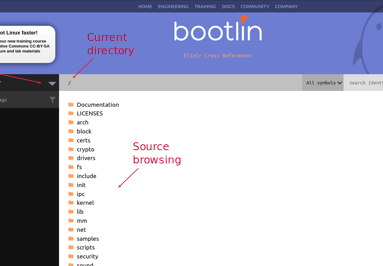
\includegraphics[height=0.5\textheight]{slides/sysdev-linux-intro-sources/elixir.pdf}
    \end{center}
  \end{columns}
\end{frame}

\begin{frame}
  \frametitle{Linux kernel size and structure}
  \begin{itemize}
  \item Linux v5.18 sources: close to 80k files, 35M lines, 1.3GiB
    % files: git ls-files | wc -l
    % lines: git ls-files | xargs cat | wc -l
    % bytes: git ls-files | xargs cat | wc -c
  \item But a compressed Linux kernel just sizes a few megabytes.
  \item So, why are these sources so big?\\
    Because they include numerous device drivers, network protocols,
    architectures, filesystems... The core is pretty small!
  \item As of kernel version v5.18 (in percentage of total number of lines):
  % Update the data by running utils/source-code-line-statistics
  % in the Linux kernel source directory
  \end{itemize}
  {\small
  \begin{columns}
    \column[t]{0.24\textwidth}
    \begin{itemize}
    \item \kdir{drivers}: 61.1\%
    \item \kdir{arch}: 11.6\%
    \item \kdir{fs}: 4.4\%
    \item \kdir{sound}: 4.1\%
    \item \kdir{tools}: 3.9\%
    \item \kdir{net}: 3.7\%
    \end{itemize}
    \column[t]{0.30\textwidth}
    \begin{itemize}
    \item \kdir{include}: 3.5\%
    \item \kdir{Documentation}: 3.4\%
    \item \kdir{kernel}: 1.3\%
    \item \kdir{lib}: 0.7\%
    \item \kdir{usr}: 0.6\%
    \item \kdir{mm}: 0.5\%
    \end{itemize}
    \column[t]{0.40\textwidth}
    \begin{itemize}
    \item \kdir{scripts}, \kdir{security}, \kdir{crypto}, \kdir{block},
      \kdir{samples}, \kdir{ipc}, \kdir{virt}, \kdir{init}, \kdir{certs}: <0.5\%
    \item Build system files: \kfile{Kbuild}, \kfile{Kconfig}, \kfile{Makefile}
    \item Other files: \kfile{COPYING}, \kfile{CREDITS},
      \kfile{MAINTAINERS}, \kfile{README}
    \end{itemize}
  \end{columns}
  }
\end{frame}
